\chapter{Microtitulación Gravimétrica Ácido-Base}\label{Sec:microfuck}
Las microtitulaciones se usaron para determinar la concentración de iones hidronio en la disolución de alimentación utilizando alícuotas muy pequeñas (alrededor de 100~$\mu$L). Esto fue necesario en los experimentos de concentración de litio a partir de agua de mar. La cantidad de la disolución de recuperación disminuía constantemente a causa de las numerosas alícuotas que se tomaron para cuantificar los cationes y no se podía disponer de grandes cantidades de esta disolución para el análisis por titulación. 

La titulación es una técnica bien establecida que permite cuantificar con gran exactitud la concentración de distintos mensurandos \citep{Skoog2013}. Las titulaciones gravimétricas presentan cualidades metrológicas mucho mejores a las titulaciones volumétricas \citep{Ahumada2018}. La poca fama de las titulaciones gravimétricas reside en el hecho de que al momento de su desarrollo, las balanzas analíticas de la época requerían protocolos largos y delicados para medir masas. Con las balanzas analíticas digitales robustas y veloces de hoy en día, las titulaciones gravimétricas representan muchas ventajas. Esta técnica debería ser implementada en alguna práctica de los laboratorios de docencia de química analítica como una forma útil de instruir a los estudiantes en metodologías analíticas de alta precisión. En el protocolo acá propuesto, la miniaturización de las cantidades de muestra de trabajo y de titulante plantean una ventaja adicional al reducir significativamente la cantidad de residuos generada.

%\begin{wrapfigure}{l}{0.49\textwidth}
%    \centering
%    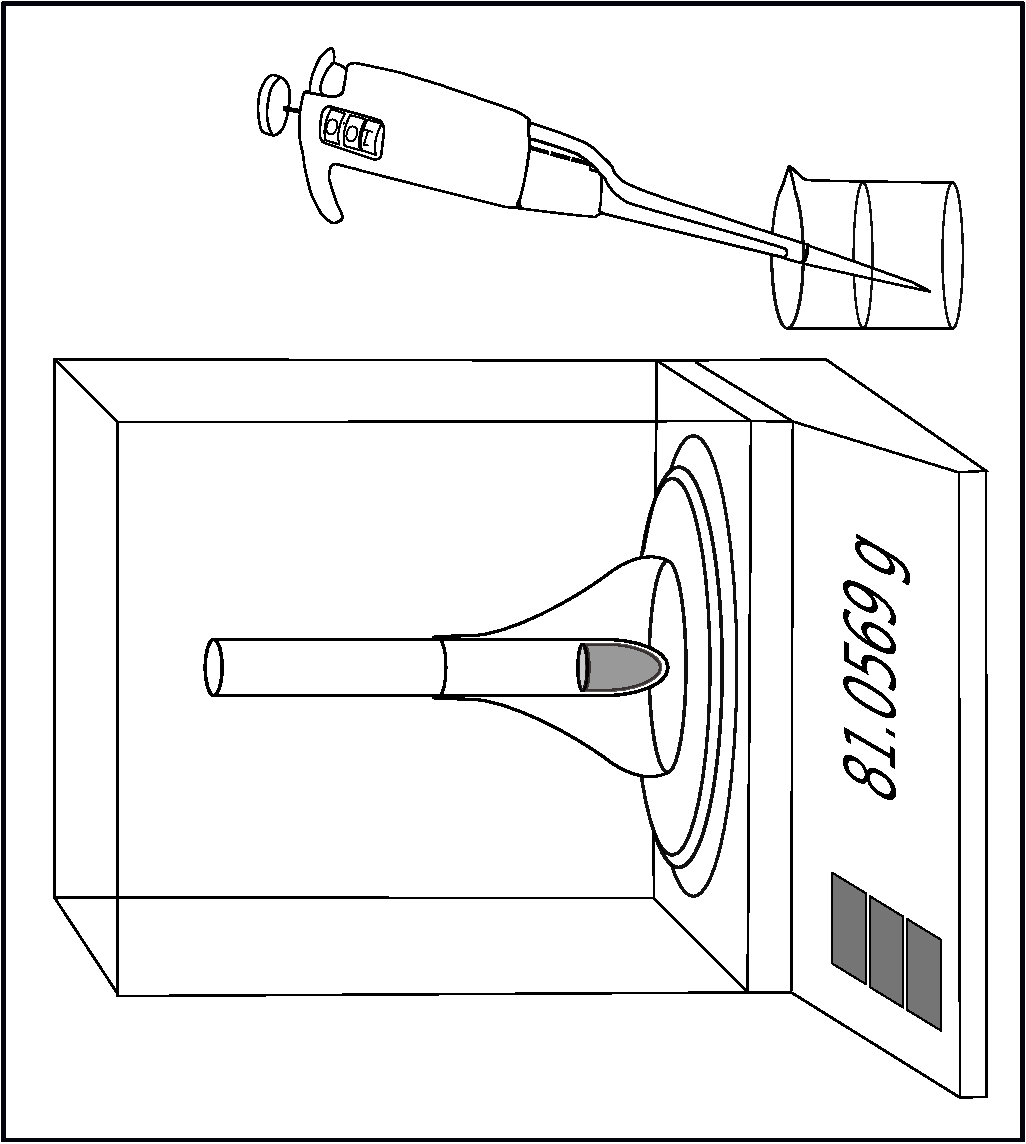
\includegraphics[height = 0.47\textwidth, angle=-90, origin=c]{App/images/Gtrit.pdf}
%    \caption{Montaje para microtitulación gravimétrica.}
%    \label{fig:celdatit}
%\end{wrapfigure}

La metodología propuesta emplea tubos de ensayo pequeños (100x13~mm) como celdas de titulación. La geometría de estas celdas resulta muy adecuada para titular pequeñas cantidades de muestra debido a la pequeña área en la que se distribuye la disolución: agitar la celda es fácil sin producir derrames, los reactivos se mezclan rápidamente y las pérdidas por evaporación disminuyen significativamente. %\footnote{Estás pérdidas por evaporación son inocuas en las titulaciones volumétricas pero se hacen reelevantes en las titulaciones gravimétricas donde la cantidad de titulante añadido hasta el punto final es cuantificado por una diferencia de masas entre la celda al comienzo y al final del proceso.} 
Para adicionar el titulante se usa una micropipeta de 10 a 100~$\mu$L. La detección de punto final se puede hacer con el indicador visual fenolftaleína disuelto al 1\% en una mezcla isopropanol/agua en proporción 1:1. Las celdas de titulación se estabilizan en el plato de la balanza usando un matraz de Erlenmeyer de 25~mL. El esquema del montaje se muestra en la Figura~\ref{fig:celdatit}.

\begin{figure}[H]
    \centering
    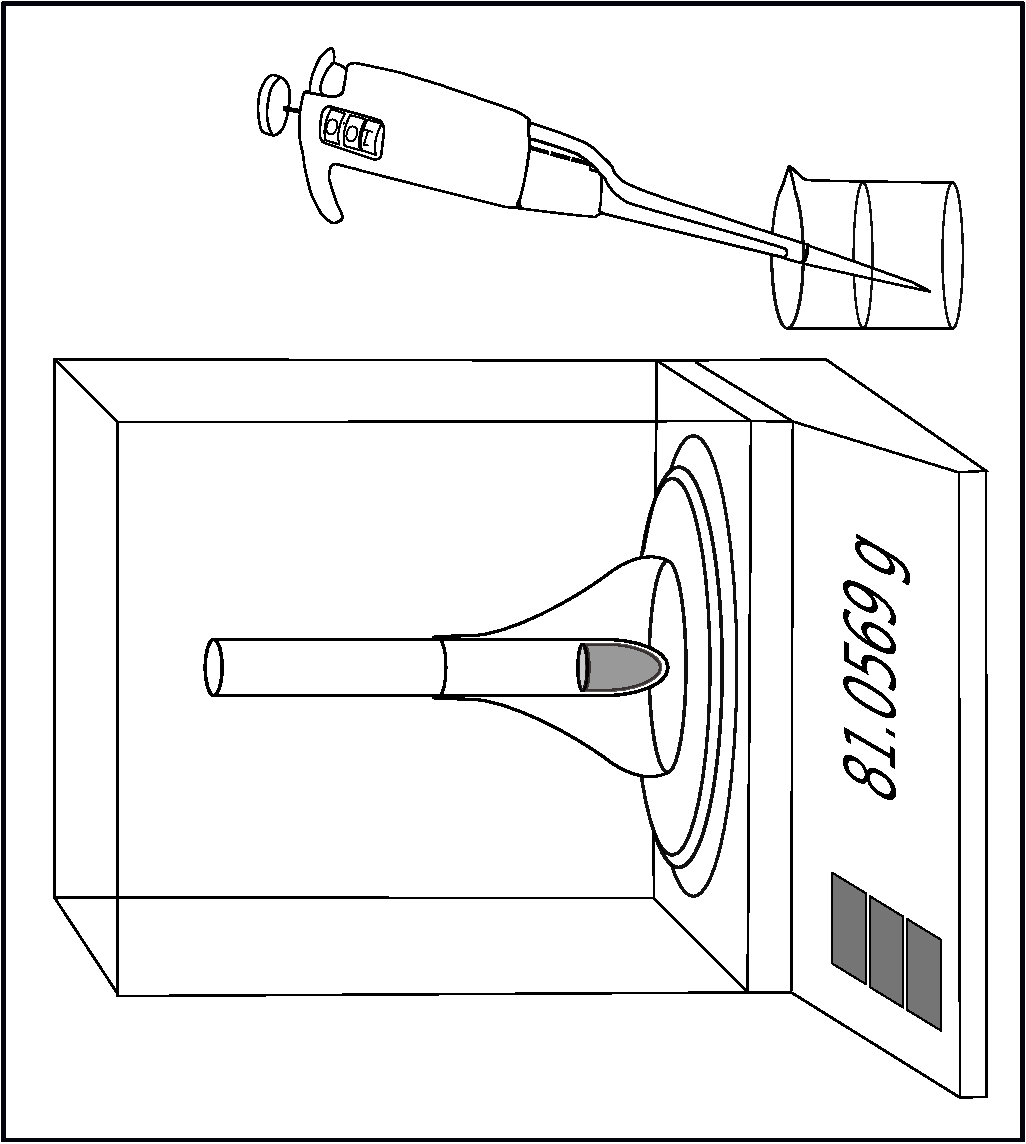
\includegraphics[height = 0.47\textwidth, angle=-90, origin=c]{App/images/Gtrit.pdf}
    \caption{Montaje para microtitulación gravimétrica.}
    \label{fig:celdatit}
\end{figure}

La masa se registra antes y después de añadir la muestra ($m_0$ y $m_s$, respectivamente), luego de añadir la disolución con indicador ($m_i$) y luego de añadir la disolución titulante hasta el punto final ($m_f$). La disolución titulante es hidróxido de sodio estandarizado ($c_{NaOH}$) con una disolución estándar de biftalato de potasio (también preparada gravimétricamente). La concentración de iones hidronio en la alícuota es:
\begin{equation}
    C_{H^+}=\frac{m_f-m_i}{m_s-m_0}c_{NaOH}
\end{equation}

Si los reactivos se añaden con cuidado de manera tal que no se pierdan en las paredes de la celda de titulación, pueden determinarse concentraciones milimolares de ácido libre en volúmenes de muestra muy pequeños que serían muy difíciles de trabajar por métodos más convencionales usando bureta. La variación del método puede ser menor al 3\%.

\ChapBib{App/App}